
The \emph{expectation maximization (EM)} algorithm (\cite{mclachlan2007algorithm, bishop2006pattern}) is a partially non-Bayesian, likelihoodist iterative method to find maximum likelihood estimates of parameters in statistical models where the model depends on latent variables.

The algorithm consist of a two step iteration where the first optimizes the variational distribution element \(Q\)  and the second optimizes the set of parameters \(\btheta\). A fully Bayesian version would consider a probability distribution over the parameter, where the distinction between the two steps disappears. In that case, as many steps as latent variables (including the parameters) are needed per iteration, where each variable is optimized at a time. For \emph{graphical models} this is easy to compute as each variable's new variational distribution depends only on its \emph{Markov blanket}, so local \emph{message passing} can be used for efficient inference (Chapter~\ref{sec:vmp}).

Using the same notation as the previous characters, EM's iterative procedure increases the ELBO for the parametric marginal \(\log P(\bx \mid \btheta)\),
\[
  \log{P(\bx \mid \btheta)} \geq \underbrace{-\E{Q(\bz)}{\log{Q(\bz)}}}_{\text{Entropy}} + \underbrace{\E{Q(\bz)}{\log{P(\bx, \bz \mid \btheta)}}}_{\text{Energy}},
\]
and the marginal likelihood \(P(\bx \mid \btheta)\) itself. Which means that aims for the value of \(\btheta\) to which the dataset better fits the model, i.e, the maximum likelihood parameter.


The EM algorithm can be viewed as two alternating maximization steps, that is, as an example of \emph{coordinate ascent} (\cite{neal1998view}). Consider the above ELBO as a function of \(Q\) and \(\btheta\):
\[
  ELBO(Q, \btheta) = -\E{Q(\bz)}{\log{Q(\bz)}} + \E{Q(\bz)}{\log{P(\bx, \bz \mid \btheta)}}.
\]
Then, the EM algorithm consists on:
\begin{itemize}
  \item For fixed \(\btheta\), choose \(Q\) such as:
    \[
    Q^{new} = \argmax_{Q}ELBO(Q, \btheta),
    \]
    which is equivalent to:
    \[
    Q^{new}(\bz) = P(\bz \mid \bx , \btheta).
    \]
  \item For fixed \(Q\), choose \(\btheta\) such as:
    \[
    \btheta^{new} = \argmax_{\btheta}ELBO(Q, \btheta).
    \]
    As \(Q\) does not depend on the parameter, this is equivalent to maximize the energy term:
    \[
    \btheta^{new} = \argmax_{\btheta} \E{Q(\bz)}{\log{P(\bx, \bz \mid \btheta)}}.
    \]
\end{itemize}

 \begin{algorithm}[t]
  \SetAlgoLined\KwData{A dataset \(\bx\) and a distribution \(P(\bx, \bz \mid \btheta)\).}
  \KwResult{Approximation of the maximum likelihood parameter.}
  Initialize \(\btheta^{(0)}\)\;
  \While{Convergence stop criteria}{
    \(Q^{(t)} = P(\bz \mid \bx, \btheta^{(t-1)})\)\;
    \(\btheta^{(t)} = \argmax_{\btheta} \E{Q^{(t)}(\bz)}{\log{P(\bx, \bz \mid \btheta)}}\)\;
  }
  \KwRet{\(\theta\)}\;
  \caption{Expectation Maximization Algorithm}\label{alg:em}
\end{algorithm}

In the specific situation where \(\bx\) consists on \(N\) observations of the same variable \(X\) and each observation of \(X\) is related with a single hidden variable \(Z\), for example, a mixture distribution, the following considerations might be taken:
\begin{itemize}\setlength{\itemsep}{0.2cm}
  \item Observations are treated as observations of i.i.d variables \(X_{1},\dots, X_{N}\) and \(Z_{1},\dots,Z_{N}\).
  \item The variational distribution \(Q\) now factorizes over the hidden variables as it is known that they are independent from each other:
    \[
    Q(\bz) = \prod_{n=1}^{N}Q(z_{n}).
    \]
    Notice that the same letter \(Q\) is being used for each variable \(Z_{n}\), this is just notational, in practice there must be a variational distribution for each of these i.i.d variables.
  \item The model distribution \(P\) factorizes over the variables as:
    \[
    P(\bx, \bz \mid \btheta) = \prod_{n=1}^{N}P(x_{n}, z_{n} \mid \btheta).
    \]
  \item The lower bound is then written as
    \[
    \begin{aligned}
      \log{P(x_{1},\dots,x_{N} \mid \btheta)} &= \sum_{n=1}^{N}\log{P(x_{n} \mid \btheta)}\\
      &\geq \sum_{n = 1}^{N} -\E{Q(z_{n})}{\log{Q(z_{n})}} + \E{Q(z_{n})}{\log{P(x_{n},z_{n} \mid \btheta)}}.
    \end{aligned}
    \]
    Where equality holds if and only if \(Q(z_{n}) = P(z_{n} \mid x_{n} , \btheta) \ \forall n=1, \dots, N\).
\end{itemize}

The procedure to optimize the parameter consists in two steps:
\begin{itemize}\setlength{\itemsep}{0.2cm}
  \item \textbf{E-step}. For fixed \(\theta\), find the distributions that maximize the above bound, i.e, choose \(Q^{new}(z_{n}) = P(z_{n} \mid x_{n} , \theta) \ \forall n = 1,\dots,N\).
  \item \textbf{M-step}. For a fixed distribution \(Q\), find the parameter \(\theta\) that maximizes the bound:
    \[
    \theta^{new} = \argmax_{\theta}\sum_{n=1}^{N}\E{Q(\bz)}{\log{P(z_{n}, x_{n} \mid \theta)}}.
    \]
\end{itemize}

\begin{exampleth}
  Consider a single variable \(X\) with \(Dom(X) = \mathbb{R}\) and a single hidden variable \(Z\) with \(dom(Z) = \{1,2\}\). Let the conditional probability be:
  \[
    P(x \mid z, \theta) = \frac{1}{\sqrt{\pi}}e^{{-(x - \theta z)}^{2}},
  \]
  and \(P(Z = 1) = P(Z = 2) = 0.5\). Suppose an observation \(x = 2.75\) we want to optimize the parameter \(\theta\) in the marginal
  \[
    P(X = 2.75 \mid \theta) = \sum_{z \in \{1,2\}} P(X = 2.75 \mid z, \theta) P(z) = \frac{1}{2\sqrt{\pi}}\big( e^{{-(2.75 - \theta)}^{2}} + e^{{-(2.75 - 2\theta)}^{2}} \big).
  \]
  Then using a distribution \(Q(z)\), the lower bound given to the log likelihood is
  \[
    \log{P(x \mid \theta)} \geq -Q(1)\log{Q(1)} - Q(2)\log{Q(2)} - \E{Q}{{(x - \theta z)}^{2}}\ + \text{const.}
  \]
  The M-step can be done analytically, noticing that due to the negative sign we want to minimize \(\E{Q}{{(x - \theta z)}^{2}}\)
  \[
    \frac{d}{d\theta}\E{Q}{{(x - \theta z)}^{2}} = \E{Q}{ 2 x z + 2\theta z^{2} } = 2x\E{Q}{z} + 2\theta \E{Q}{z^{2}} = 0 \iff \theta = \frac{x\E{Q}{z}}{\E{Q}{z^{2}}},
  \]
  \[
    \frac{d^{2}}{d^{2}\theta}\E{Q}{{(x - \theta z)}^{2}} = 2\E{Q}{z^{2}} \geq 0,
  \]
  so the new parameter optimal parameter is
  \[
    \theta_{new} = x \frac{\E{Q}{z}}{\E{Q}{z^{2}}}.
  \]

  The E-step would set \(Q_{new}(z) = P(z \mid x , \theta)\), in this case
  \[
    \begin{aligned}
      Q^{new}(Z = 1) &= \frac{P(X = 2.75 \mid Z = 1, \theta)P(Z = 1)}{P(X = 2.75)} = \frac{e^{-(2.75-\theta)}}{ e^{-(2.75-\theta)} + e^{-(2.75-2\theta)}  },\\
      Q^{new}(Z = 2) &= \frac{P(X = 2.75 \mid Z = 2, \theta)P(Z = 2)}{P(X = 2.75)} = \frac{e^{-(2.75-2\theta)}}{ e^{-(2.75-\theta)} + e^{-(2.75-2\theta)}  }.
    \end{aligned}
  \]
\end{exampleth}



\section{EM increases the marginal likelihood}

It is clear that the EM algorithm does increase the lower bound in each iteration but also the marginal likelihood.

\begin{proposition}
  The log likelihood \(P(x \mid \btheta)\) is not decreased in each iteration of the EM algorithm, i.e, if \(\btheta^{old}\) and \(\btheta^{new}\) are two consecutive values of the parameter, EM verifies:
  \[
    \log{P(\bx \mid \btheta^{new})} - \log{P(\bx \mid \btheta^{old})} \geq 0.
  \]
\end{proposition}
\begin{proof}
As a result of the E-step \(Q\) is set to
\[
  Q(\bz) = P(\bz \mid \bx, \btheta^{old}).
\]
So the lower bound in terms of \(\btheta^{old}\) and \(\btheta^{new}\) is
\[
  ELBO(\btheta^{new} \mid \btheta^{old}) =  \underbrace{-\E{P(\bz \mid \bx, \btheta^{old})}{\log{P(\bz \mid \bx, \btheta^{old})}}}_{\text{Entropy}} + \underbrace{\E{P(\bz \mid \bx, \btheta^{old})}{\log{P(\bz,\bx \mid \btheta^{new})}}}_{\text{Energy}}.
\]
From the definition of the Kullback-Leibler divergence we get that
\[
  \log{P(\bx \mid \btheta^{new})} = ELBO(\btheta^{new}\mid \btheta^{old}) + \KL{P(\bz \mid \bx, \btheta^{old})}{P(\bz \mid \bx, \btheta^{new})}.
\]
We could use \(\btheta^{old}\) in the above formula getting
\[
  \log{P(\bx \mid \btheta^{old})} = ELBO(\btheta^{old} \mid \btheta^{old}) + \KL{P(\bz \mid \bx, \btheta^{old})}{P(\bz \mid \bx, \btheta^{old})} = ELBO(\btheta^{old} \mid \btheta^{old}).
\]
So we can compute the difference between the log likelihood between two consecutive iterations as
\[
  \begin{aligned}
    \log{P(\bx \mid \btheta^{new})} - \log{P(\bx \mid \btheta^{old})} &= ELBO(\btheta^{new}\mid \btheta^{old}) - ELBO(\btheta^{old} \mid \btheta^{old})\\
    &+  \KL{P(\bz \mid \bx, \btheta^{old})}{P(\bz \mid \bx, \btheta^{new})}.
  \end{aligned}
\]
Where we know the last term is always positive. About the difference of bounds, the M-step ensures the new parameter makes the lower bound higher or equal to the current one, so that difference is also positive.
\[
   \log{P(\bx \mid \btheta^{new})} - \log{P(\bx \mid \btheta^{old})} \geq 0.
 \]
\end{proof}


\section{Example: Binomial Mixture}
In this section we are using a coin-flipping experiment as an example to show limitations of classical maximum likelihood inference due to the presence of hidden variables. The EM algorithm is then used to surpass these limitations. The example consists in a \emph{mixture distribution} based on~\cite{do2008expectation}.

The experiment consist of randomly choosing one of a pair of coins \(A\) and \(B\) with unknown biases, \(\theta_{A}\)  and \(\theta_{B}\). Let \(1\) denote \textit{heads} and \(0\) denote \textit{tails}. The selected coin is tossed \(M\)  times, repeating this whole procedure \(N\)  times. In short, the experiment is governed by two parameters:
\[
  P(A = 1) = \theta_{A} \quad \text{and} \quad P(B = 1) = \theta_{B},
\]

Maximum likelihood training attempts to infer the value of \(\bm{\theta} = (\theta_{A}, \theta_{B})\) that maximizes the likelihood.

Given that the maximum likelihood distribution is the empirical distribution:
\[
  \theta_{A}^{ML} = \frac{\text{Heads of coin }A}{\text{Total flips of coin }A} \quad \text{and} \quad \theta_{B}^{ML} = \frac{\text{Heads of coin }B}{\text{Total flips of coin }B}.
\]

Consider now that the identity of the coin that is being flipped is unknown. Let \(X\) be the random variable modeling the number of heads in \(M\) flips and \(Z\) the coin being flipped. In this situation, using the empirical distribution is not possible as the identity of the coin is unknown. In this kind of situations, the EM algorithm performs maximum likelihood training while dealing with the hidden variable.


The conditional \(x_{n} \mid z_{n}, \btheta\) follows a Bernoulli distribution:
\[
  x_{n} \mid z_{n}, \btheta \sim B(M, \theta_{z_{n}}) \implies P(x_{n} \mid z_{n}, \btheta) = \binom{M}{x_{n}}\theta_{z_{n}}^{x_{n}}{(1-\theta_{z_{n}})}^{M - x_{n}} \ \forall n =1,\dots,N,
\]
and the probability of choosing a coin is \(P(z_{n}=A) = P(z_{n}=B)=0.5 \; \forall n =1,\dots,N\).

The lower bound is:
\[
  \sum_{n=1}^{N}\log{P(x_{n} \mid \bm{\theta})} \geq \sum_{n=1}^{N}-\E{Q(z_{n})}{\log{Q(z_{n})}} + \E{Q(z_{n})}{\log{P(z_{n}, x_{n} \mid \bm{\theta})}},
\]

The \textbf{E-step} consists on setting (given a fixed \(\theta\), which is not considered a random variable),
\[
  \begin{aligned}
    Q(z_{n}) &= P(z_{n} \mid x_{n}, \bm{\theta}) = \frac{P(x_{n} \mid z_{n}, \bm{\theta})P(z_{n})}{P(x_{n})} \\
    &= \frac{0.5\ \theta_{z_{n}}^{x_{n}}{(1-\theta_{z_{n}})}^{M - x_{n}}}{\int_{z_{n}}P(x_{n},z_{n}\mid \btheta)}\\
    &= \frac{P(z_{n})\theta_{z_{n}}^{x_{n}}{(1-\theta_{z_{n}})}^{M - x_{n}}}{\int_{z_{n}, \btheta}P(x_{n}\mid z_{n}, \btheta)P(z_{n})}\\
    &= \frac{\theta_{z_{n}}^{x_{n}}{(1-\theta_{z_{n}})}^{M - x_{n}}}{  \theta_{A}^{x_{n}}{(1-\theta_{A})}^{M - x_{n}} + \theta_{B}^{x_{n}}{(1-\theta_{B})}^{M - x_{n}}} \quad \forall n=1,\dots,N.
  \end{aligned}
\]

On the other hand, the \textbf{M-step} consists on setting
\[
  \begin{aligned}
    \bm{\theta}^{new} &= \argmax_{\theta} \sum_{n=1}^{N}\E{Q(z_{n})}{\log P(x_{n}, z_{n} \mid \btheta)}\\
    &= \argmax_{\theta} \sum_{n=1}^{N}\E{Q(z_{n})}{\log P(x_{n} \mid z_{n}, \btheta)P(z_{n})}\\
    &= \argmax_{\theta} \sum_{n=1}^{N}\E{Q(z_{n})}{\log P(x_{n} \mid z_{n}, \btheta)}
  \end{aligned}
\]
where in the last equality we used that \(P(z_{n}) = 0.5\) is constant. The expectation is written as
\[
  \begin{aligned}
    \E{Q(z_{n})}{\log P(x_{n} \mid z_{n}, \btheta)} &= Q(z_{n} = A)\Big( x_{n}\log{\theta_{A}} + (M - x_{n})\log{(1 - \theta_{A})} \Big)\\
    &+ Q(z_{n} = B)\Big( x_{n}\log{\theta_{B}} + (M - x_{n})\log{(1 - \theta_{B})} \Big).
  \end{aligned}
\]
As \(\theta_{A}\) and \(\theta_{B}\) are separated in each term, the optimum can be found separately, the term affected by \(\theta_{A}\) is
\[
  \sum_{n=1}^{N} Q(z_{n}=A) \Big(x_{n}\log{\theta_{A}} + (M - x_{n})\log{(1-\theta_{A})}\Big),
\]
deriving and setting to \(0\) we get the following maxima.
\[
  \sum_{n=1}^{N}Q(z_{n}=A)\Big(\frac{x_{n}}{\theta_{A}} - \frac{M - x_{n}}{1- \theta_{A}}\Big) = 0 \iff \theta_{A} = \sum_{n=1}^{N}Q(z_{n}=A)\frac{x_{n}}{M}.
\]
The same argument is valid for \(\theta_{B}\).

\begin{figure}
  \centering
  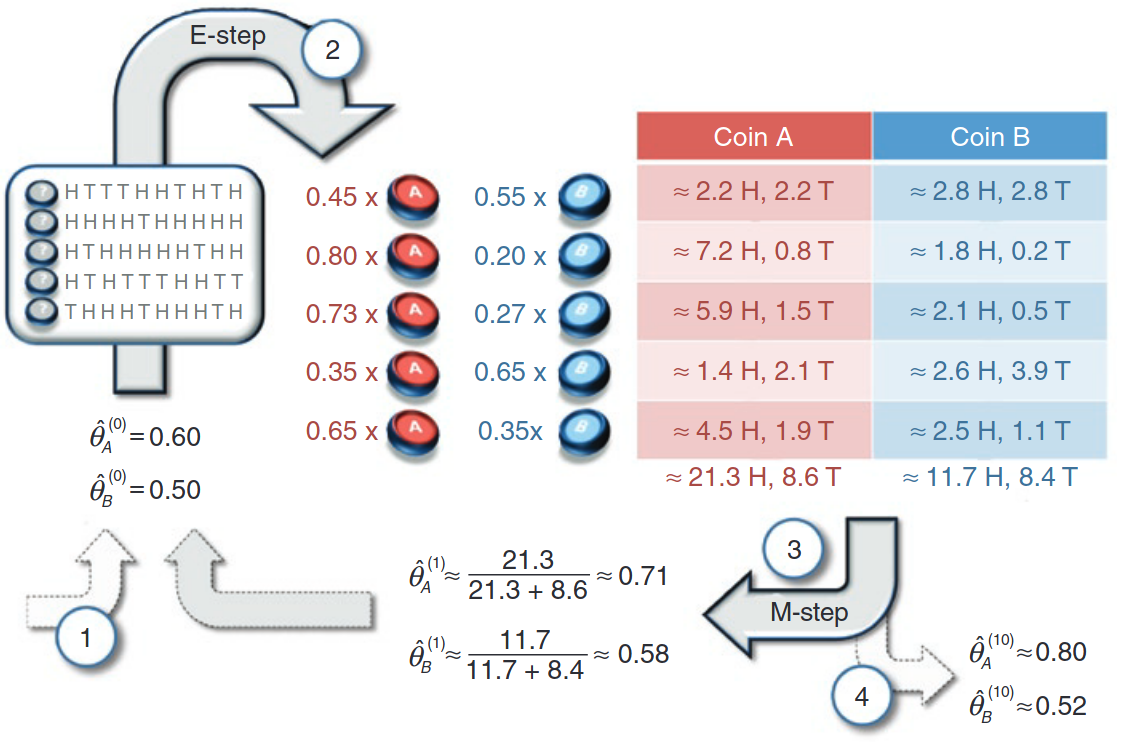
\includegraphics[width=0.7\textwidth]{tex/images/mixture}
  \caption{EM algorithm step in Mixture~\cite{do2008expectation}}\label{fig:mixture}
\end{figure}

We are know using the figure~\ref{fig:mixture} to set the example in a numerical context. We are following the given data points in the diagram.
\begin{enumerate}
  \item We are considering a prior \(\bm{\theta} = (0.6, 0.5)\), a set of \(N = 5\) samples and \(M = 10\) flips per sample.
  \item In the \textbf{E-step}, we calculate each \(Q(z_{n})\).
    \[
    \begin{aligned}
      Q(z_{1} = A) &= \frac{0.6^{5} 0.4^{5}}{0.6^{5}0.4^{5} + 0.5^{5}0.5^{5}} \approx 0.45 \implies Q(z_{1} = B) \approx 0.55,\\
      &\mathrel{\makebox[\widthof{=}]{\vdots}} \\
      Q(z_{5} = A) &\approx 0.65 \implies Q(z_{5}=B) \approx 0.35.
    \end{aligned}
    \]
  \item The \textbf{M-step} is then:
    \[
    \begin{aligned}
      \theta_{A} &= \sum_{n=1}^{5}Q(z_{n})\frac{x_{n}}{10} \approx \frac{21.3}{21.3 + 8.6} \approx 0.71,\\
      \theta_{B} &\approx 0.58.
    \end{aligned}
    \]
  \item Step 4 represents a possible solution after \(10\) iterations.
\end{enumerate}


\section{Partial steps}

Making a partial M-step consist on not using the optimal parameter for the energy term, but using one with just higher energy. Finding this values can be easier than finding the optimal one and convergence still follows as the only requirement to make the likelihood increase was to increase the lower bound.

On the other hand, when studying the increase on the likelihood, we supposed that the optimal E-step was being used. It cannot be guarantee that a partial step would increase the likelihood in this case, even though it does increase the lower bound.

Another important factor is, that the EM algorithm assumes that the energy term is possible to calculate, which may not be. As an approach to solve this situation, we can set a class of distributions \(\mathcal{Q}\), and minimize the Kullback-Leibler divergence between \(P(\bz \mid \bx, \theta)\) and a distribution \(Q \in \mathcal{Q}\), so we pick a distribution such that
\[
  Q = \argmin_{Q \in \mathcal{Q}} \KL{Q(\bz)}{P(\bz\mid \bx, \theta)}.
\]

An extreme case is to choose \(\mathcal{Q}\) as delta functions, where the energy term is now a constant, and the optimal setting is
\[
Q(z_{n}) = \delta (z_{n}, z_{n}^{opt}) , \quad z_{n}^{opt} = \argmax_{z}P(z , x_{n} \mid \theta).
\]
This is called \emph{Viterbi training} and does not guarantee that the log likelihood is being increased in each iteration.
